\chapter{The Fourier Transform of a Constant}
\label{ch:constant}

\begin{quote}
\itshape
A signal that never changes should contain only the frequency $\omega=0$. The claim is
uncontroversial. The integral that is supposed to express it does not converge. This chapter
separates the two facts, computes what can be computed, and identifies exactly what has to be
added to the language in order to write the answer.
\end{quote}

\section{Conventions and the elementary theory}

Throughout,
\begin{equation}
\F[f](\omega)=\fh(\omega)=\int_{\R} f(t)e^{-i\omega t}\dd t ,
\qquad
f(t)=\frac{1}{2\pi}\int_{\R}\fh(\omega)e^{i\omega t}\dd\omega .
\label{eq:ftpair}
\end{equation}
The second formula is not assumed; it is proved in Chapter~\ref{ch:tespered} under hypotheses that
cover everything used here. Until then, any use of it is flagged.

The kernel $e^{-i\omega t}$ is a \emph{frequency probe}. Multiplying a signal by it and integrating
compares the signal with a pure oscillation of frequency $\omega$: when the two agree in frequency
the product is a constant and the contributions add; otherwise they rotate and cancel. This is a
correct description of what the integral \emph{measures}. It is not an argument that the integral
converges, and the distinction is the whole content of the next section.

\begin{proposition}[the $L^{1}$ theory]\label{prop:L1}
Let $f\in\Lone$. Then
\begin{enumerate}
\item the integral in \eqref{eq:ftpair} converges absolutely for every $\omega$, and
\begin{equation}
\|\fh\|_{\infty}\le\|f\|_{1};
\label{eq:L1bound}
\end{equation}
\item $\fh$ is uniformly continuous on $\R$;
\item $\fh(\omega)\to 0$ as $|\omega|\to\infty$ \textup{(Riemann--Lebesgue)}.
\end{enumerate}
\end{proposition}

\begin{proof}
(i) Since $|e^{-i\omega t}|=1$, the integrand is dominated by $|f(t)|$, which does not depend on
$\omega$ and is integrable; \eqref{eq:L1bound} follows by taking suprema. (ii) and (iii) are the
standard consequences of the continuity of translation in $L^{1}$ and of the density of step
functions; both are quoted.
\end{proof}

\begin{example}
$f\equiv 1$ is not in $\Lone$, so Proposition~\ref{prop:L1} says nothing about it. It is worth
insisting on what this does and does not mean: membership in $\Lone$ is a \emph{sufficient}
condition for the transform to exist as an absolutely convergent integral, and its failure is not
a proof that every conceivable interpretation diverges. To decide the question one has to compute.
\end{example}

Two properties of the transform will be used constantly and are recorded once.

\begin{proposition}[elementary symmetries]\label{prop:symmetries}
For any $f$ for which the integrals make sense,
\begin{align}
\F[f(\cdot-a)](\omega)&=e^{-ia\omega}\fh(\omega), \label{eq:timeshift}\\
\F[e^{i\omega_{0}t}f(t)](\omega)&=\fh(\omega-\omega_{0}), \label{eq:modulation}\\
\F[f(a\,\cdot)](\omega)&=\frac{1}{|a|}\,\fh\!\left(\frac{\omega}{a}\right),\qquad a\neq0.
\label{eq:dilation}
\end{align}
If $f$ is real then $\overline{\fh(\omega)}=\fh(-\omega)$; if $f$ is even (odd) then $\fh$ is even
(odd); if $f$ is real and even then $\fh$ is real and even.
\end{proposition}

\begin{proof}
\eqref{eq:timeshift} and \eqref{eq:modulation} are changes of variable in the exponent.
For \eqref{eq:dilation} substitute $t=as$:
\begin{equation}
\int_{\R}f(at)e^{-i\omega t}\dd t
=\frac{1}{|a|}\int_{\R}f(s)e^{-i(\omega/a)s}\dd s
=\frac{1}{|a|}\fh\!\left(\frac{\omega}{a}\right).
\end{equation}
The symmetry statements follow by conjugating and by substituting $t\mapsto-t$.
\end{proof}

\section{The truncated integral, and why it fails}

Let $f\equiv1$. Formally,
\begin{equation}
\fh(\omega)=\int_{\R}e^{-i\omega t}\dd t .
\label{eq:badintegral}
\end{equation}
To give the expression a chance, truncate symmetrically and compute. This is the most favourable
truncation available, so if it fails, all the others fail too.

\begin{lemma}\label{lem:IT}
For $T>0$ and $\omega\in\R$,
\begin{equation}
I_{T}(\omega):=\int_{-T}^{T}e^{-i\omega t}\dd t=
\begin{cases}
\dfrac{2\sin(\omega T)}{\omega}, & \omega\neq0,\\[8pt]
2T, & \omega=0 .
\end{cases}
\label{eq:IT}
\end{equation}
The function $\omega\mapsto I_{T}(\omega)$ is continuous at $\omega=0$.
\end{lemma}

\begin{proof}
For $\omega\neq0$,
\begin{equation}
\int_{-T}^{T}e^{-i\omega t}\dd t
=\left[\frac{e^{-i\omega t}}{-i\omega}\right]_{-T}^{T}
=\frac{e^{-i\omega T}-e^{i\omega T}}{-i\omega}
=\frac{2\sin(\omega T)}{\omega},
\end{equation}
using $\sin x=(e^{ix}-e^{-ix})/(2i)$. For $\omega=0$ the integrand is $1$ and the integral is
$2T$. Continuity at $0$ follows from $\lim_{\omega\to0}\sin(\omega T)/\omega=T$.
\end{proof}

\begin{proposition}\label{prop:nolimit}
Fix $\omega\neq0$. Then $I_{T}(\omega)$ has no limit as $T\to\infty$.
\end{proposition}

\begin{proof}
Put $a=|\omega|>0$. For $n=0,1,2,\dots$ set
\begin{equation}
T_{n}=\frac{\pi/2+2\pi n}{a},
\qquad
S_{n}=\frac{3\pi/2+2\pi n}{a}.
\end{equation}
Then $aT_{n}=\pi/2+2\pi n$ and $aS_{n}=3\pi/2+2\pi n$, so $\sin(aT_{n})=1$ and $\sin(aS_{n})=-1$.
Since $\sin(\omega T)=\pm\sin(aT)$ according to the sign of $\omega$, one gets
\begin{equation}
\frac{2\sin(\omega T_{n})}{\omega}=\pm\frac{2}{a},
\qquad
\frac{2\sin(\omega S_{n})}{\omega}=\mp\frac{2}{a}.
\end{equation}
Both sequences of truncation lengths tend to infinity, while the values stay at two different
numbers. Hence no limit exists.
\end{proof}

At $\omega=0$ the behaviour is different but equally unusable: $I_{T}(0)=2T\to+\infty$. So the
zero frequency does not produce a value either; it produces unbounded growth.

\begin{remark}[three statements, only one of which is correct]
\emph{Wrong:} ``for $\omega\neq0$ the integral equals $0$''. The integral does not exist, so it
cannot equal anything. \emph{Wrong:} ``at $\omega=0$ the transform is infinite'', since $\infty$ is
not a value. \emph{Correct:} for every fixed $\omega\neq0$ the truncated integral oscillates
without limit, and at $\omega=0$ it grows without bound; therefore \eqref{eq:badintegral} is not a
convergent improper integral.
\end{remark}

\begin{remark}[an object worth keeping]\label{rem:sinc}
The function $I_{T}$ is not garbage. It is the Fourier transform of the rectangular window
$w_{T}=\mathbf{1}_{[-T,T]}$, and it will reappear in Chapter~\ref{ch:tespered} as an example of a
family that fails every pointwise test but converges in the distributional sense. The failure
recorded here is a failure of one notion of convergence, not of the object.
\end{remark}

\section{Regularization by a two-sided exponential}

The strategy changes. Instead of evaluating \eqref{eq:badintegral}, we construct a family of
functions that are integrable, computable, and converge to the constant, and we examine where their
transforms go.

For $\ep>0$ set
\begin{equation}
f_{\ep}(t)=e^{-\ep|t|}.
\label{eq:feps}
\end{equation}
Then
\begin{equation}
\|f_{\ep}\|_{1}=\int_{\R}e^{-\ep|t|}\dd t=\frac{2}{\ep}<\infty,
\qquad
f_{\ep}(t)\to1\quad\text{for every fixed }t,
\label{eq:feps-approx}
\end{equation}
so Proposition~\ref{prop:L1} applies to each member of the family. The parameter has a transparent
meaning: $f_{\ep}$ decays on the time scale $1/\ep$, so that as $\ep\downarrow0$ it stays close to
$1$ on ever longer intervals.

\begin{theorem}\label{thm:exptransform}
For every $\ep>0$ and every $\omega\in\R$,
\begin{equation}
\F\big[e^{-\ep|\cdot|}\big](\omega)
=\frac{1}{\ep-i\omega}+\frac{1}{\ep+i\omega}
=\frac{2\ep}{\ep^{2}+\omega^{2}}
=:G_{\ep}(\omega).
\label{eq:Geps}
\end{equation}
\end{theorem}

\begin{proof}
The absolute value changes expression at $t=0$, so split the integral:
\begin{equation}
\int_{\R}e^{-\ep|t|}e^{-i\omega t}\dd t
=\int_{-\infty}^{0}e^{(\ep-i\omega)t}\dd t+\int_{0}^{\infty}e^{-(\ep+i\omega)t}\dd t .
\end{equation}
On the left half line, $|t|=-t$ and the exponent is $(\ep-i\omega)t$, whose real part $\ep$ is
positive; hence
\begin{equation}
\int_{-\infty}^{0}e^{(\ep-i\omega)t}\dd t
=\left[\frac{e^{(\ep-i\omega)t}}{\ep-i\omega}\right]_{-\infty}^{0}
=\frac{1}{\ep-i\omega},
\end{equation}
the lower boundary term vanishing because $|e^{(\ep-i\omega)t}|=e^{\ep t}\to0$ as $t\to-\infty$.
Similarly, on the right half line the real part of $-(\ep+i\omega)$ is $-\ep<0$, so
\begin{equation}
\int_{0}^{\infty}e^{-(\ep+i\omega)t}\dd t
=\left[\frac{e^{-(\ep+i\omega)t}}{-(\ep+i\omega)}\right]_{0}^{\infty}
=\frac{1}{\ep+i\omega}.
\end{equation}
Adding and putting over a common denominator,
\begin{equation}
\frac{1}{\ep-i\omega}+\frac{1}{\ep+i\omega}
=\frac{(\ep+i\omega)+(\ep-i\omega)}{(\ep-i\omega)(\ep+i\omega)}
=\frac{2\ep}{\ep^{2}+\omega^{2}}. \qedhere
\end{equation}
\end{proof}

\begin{remark}[checks that cost nothing]
The computation should be checked against the symmetries of Proposition~\ref{prop:symmetries}.
Since $f_{\ep}$ is real and even, $G_{\ep}$ must be real, even, and nonnegative; it is. The value
at the origin is $G_{\ep}(0)=2/\ep$, which blows up as $\ep\downarrow0$, consistent with the
divergence at zero frequency found in Proposition~\ref{prop:nolimit}. Finally, if $\omega$ is
allowed to be complex, $G_{\ep}$ has poles at $\omega=\pm i\ep$, and these poles approach the real
axis as $\ep\downarrow0$; this is the analytic picture of ``the mass landing on $\omega=0$''. It is
a useful mnemonic, not an argument.
\end{remark}

\section{Peak, width, area}

Three numbers describe the family $G_{\ep}$ completely, and each of them has a definite limit
behaviour.

\begin{proposition}\label{prop:three}
For $\ep>0$,
\begin{equation}
G_{\ep}(0)=\frac{2}{\ep},
\qquad
\operatorname{FWHM}\big(G_{\ep}\big)=2\ep,
\qquad
\int_{\R}G_{\ep}(\omega)\dd\omega=2\pi .
\label{eq:three}
\end{equation}
\end{proposition}

\begin{proof}
The first is immediate. For the second, the half maximum is $\tfrac12 G_{\ep}(0)=1/\ep$, so the
half-maximum points satisfy
\begin{equation}
\frac{2\ep}{\ep^{2}+\omega^{2}}=\frac{1}{\ep}
\iff \ep^{2}+\omega^{2}=2\ep^{2}
\iff |\omega|=\ep ,
\end{equation}
and the full width is $2\ep$. For the third,
\begin{equation}
\int_{\R}\frac{2\ep}{\ep^{2}+\omega^{2}}\dd\omega
=2\ep\cdot\frac{1}{\ep}\left[\arctan\frac{\omega}{\ep}\right]_{-\infty}^{\infty}
=2\left(\frac{\pi}{2}+\frac{\pi}{2}\right)=2\pi . \qedhere
\end{equation}
\end{proof}

Thus the peak grows like $\ep^{-1}$, the width shrinks like $\ep$, and the area is independent of
$\ep$. The product of height and width is constant, which is the quantitative form of the phrase
``spreading in time forces concentration in frequency''. The next proposition makes the mechanism
exact and shows that it is a single identity rather than a collection of coincidences.

\begin{proposition}[dilation]\label{prop:dilation}
Let $g\in\Lone$ and $a>0$. If $f(t)=g(t/a)$ then
\begin{equation}
\fh(\omega)=a\,\widehat{g}(a\omega).
\label{eq:dilate}
\end{equation}
Applied to $g(t)=e^{-|t|}$, whose transform is $2/(1+\omega^{2})$, this gives
\begin{equation}
G_{\ep}(\omega)=\frac{1}{\ep}\cdot\frac{2}{1+(\omega/\ep)^{2}}
=\frac{2\ep}{\ep^{2}+\omega^{2}},
\end{equation}
in agreement with Theorem~\ref{thm:exptransform}.
\end{proposition}

\begin{proof}
Substitute $t=as$, $\dd t=a\dd s$:
\begin{equation}
\fh(\omega)=\int_{\R}g(t/a)e^{-i\omega t}\dd t
=a\int_{\R}g(s)e^{-i\,a\omega\,s}\dd s=a\,\widehat{g}(a\omega). \qedhere
\end{equation}
\end{proof}

\begin{remark}[what the area is not]
The constant value $2\pi$ of the area is a property of this particular family, not a conservation
law. The genuine conservation law is Plancherel's identity
$\|f\|_{2}^{2}=(2\pi)^{-1}\|\fh\|_{2}^{2}$, and it is inapplicable here in the limit: for
$f_{\ep}$,
\begin{equation}
\|f_{\ep}\|_{2}^{2}=\int_{\R}e^{-2\ep|t|}\dd t=\frac{1}{\ep}\longrightarrow\infty ,
\end{equation}
so the constant function is not a finite-energy signal and cannot be treated as an $L^{2}$ limit.
This is worth remembering whenever ``the area of the spectrum'' is mentioned.
\end{remark}

\begin{figure}[t]
\centering
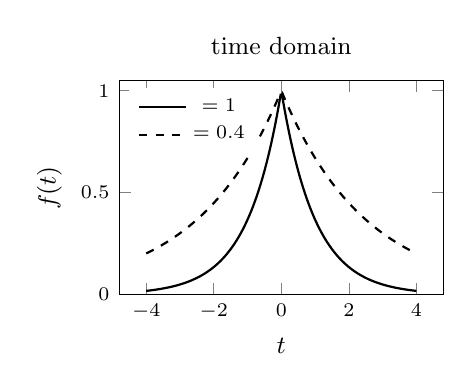
\begin{tikzpicture}
\begin{axis}[width=0.47\textwidth,height=4.3cm,domain=-4:4,samples=200,
  ymin=0,ymax=1.05,xlabel={$t$},ylabel={$f_{\ep}(t)$},
  title={\small time domain},
  legend style={font=\scriptsize,at={(0.03,0.97)},anchor=north west,draw=none},
  ticklabel style={font=\scriptsize},label style={font=\small}]
\addplot[thick,black] {exp(-1*abs(x))};
\addplot[thick,black,dashed] {exp(-0.4*abs(x))};
\legend{$\ep=1$,$\ep=0.4$}
\end{axis}
\end{tikzpicture}\hfill
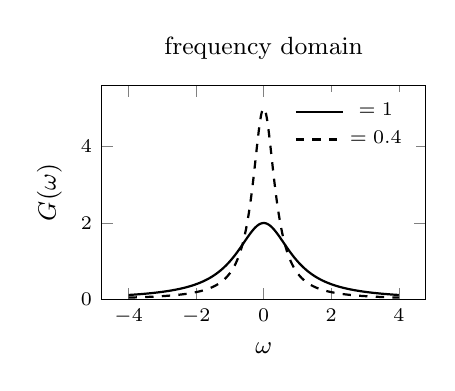
\begin{tikzpicture}
\begin{axis}[width=0.47\textwidth,height=4.3cm,domain=-4:4,samples=400,
  ymin=0,ymax=5.6,xlabel={$\omega$},ylabel={$G_{\ep}(\omega)$},
  title={\small frequency domain},
  legend style={font=\scriptsize,at={(0.97,0.97)},anchor=north east,draw=none},
  ticklabel style={font=\scriptsize},label style={font=\small}]
\addplot[thick,black] {2*1/(1+x^2)};
\addplot[thick,black,dashed] {2*0.4/(0.16+x^2)};
\legend{$\ep=1$,$\ep=0.4$}
\end{axis}
\end{tikzpicture}
\caption{The same two parameters seen in both domains. The vertical scales differ: the dashed
curve has peak $2/0.4=5$.}
\end{figure}

\section{The normalized kernel and the sampling property}

The family $G_{\ep}$ has total mass $2\pi$. The factor is an artefact of the normalization
\eqref{eq:ftpair} and is removed once and for all.

\begin{definition}\label{def:Keps}
For $\ep>0$ let
\begin{equation}
K_{\ep}(x)=\frac{1}{\pi}\frac{\ep}{x^{2}+\ep^{2}},
\qquad\text{so that}\qquad
K_{\ep}=\frac{G_{\ep}}{2\pi},\qquad \int_{\R}K_{\ep}\dd x=1 .
\label{eq:Keps}
\end{equation}
\end{definition}

\begin{proposition}[mass concentrates at the origin]\label{prop:concentration}
For every $a>0$,
\begin{equation}
\int_{-a}^{a}K_{\ep}(x)\dd x=\frac{2}{\pi}\arctan\frac{a}{\ep}\longrightarrow1
\qquad(\ep\downarrow0).
\label{eq:concentration}
\end{equation}
\end{proposition}

\begin{proof}
Immediate from the antiderivative of $1/(x^{2}+\ep^{2})$; the limit uses
$\arctan y\to\pi/2$ as $y\to\infty$.
\end{proof}

The quantifier order in \eqref{eq:concentration} matters: $a$ is fixed first, and only then does
$\ep$ tend to zero. Equivalently: for every fixed interval around the origin, no matter how short,
the fraction of the total mass inside it tends to one.

\begin{theorem}[sampling]\label{thm:sampling}
Let $\varphi$ be bounded and continuous at $0$. Then
\begin{equation}
\int_{\R}K_{\ep}(x)\varphi(x)\dd x\longrightarrow\varphi(0)
\qquad(\ep\downarrow0).
\label{eq:sampling}
\end{equation}
\end{theorem}

\begin{proof}
Since $\int K_{\ep}=1$, the error is
\begin{equation}
\int_{\R}K_{\ep}(x)\varphi(x)\dd x-\varphi(0)
=\int_{\R}K_{\ep}(x)\big[\varphi(x)-\varphi(0)\big]\dd x .
\end{equation}
Let $\eta>0$. By continuity at $0$ there is $a>0$ with $|\varphi(x)-\varphi(0)|<\eta$ whenever
$|x|<a$. Splitting at $|x|=a$ and using $K_{\ep}\ge0$,
\begin{equation}
\left|\int_{\R}K_{\ep}\big[\varphi(\cdot)-\varphi(0)\big]\right|
\le\eta\int_{|x|<a}K_{\ep}
+2\|\varphi\|_{\infty}\int_{|x|\ge a}K_{\ep}
\le\eta+2\|\varphi\|_{\infty}\Big(1-\frac{2}{\pi}\arctan\frac{a}{\ep}\Big).
\end{equation}
Fix $a$ and let $\ep\downarrow0$: the second term tends to $0$ by
Proposition~\ref{prop:concentration}. Hence
\begin{equation}
\limsup_{\ep\to0}\Big|\int_{\R}K_{\ep}\varphi-\varphi(0)\Big|\le\eta ,
\end{equation}
and $\eta>0$ was arbitrary.
\end{proof}

A second proof, which is often shorter in practice, removes the varying scale by a change of
variable. Substituting $x=\ep u$ in the definition of $K_{\ep}$ gives
\begin{equation}
\int_{\R}K_{\ep}(x)\varphi(x)\dd x
=\frac{1}{\pi}\int_{\R}\frac{\varphi(\ep u)}{1+u^{2}}\dd u ,
\label{eq:substitution-proof}
\end{equation}
and now the weight $(1+u^{2})^{-1}/\pi$ is fixed and the parameter has migrated into the test
function. The integrand is dominated by $\|\varphi\|_{\infty}/(\pi(1+u^{2}))$, which is integrable
and independent of $\ep$; dominated convergence applies directly and gives $\varphi(0)$. The two
proofs are the same estimate seen from two sides, and the second one will be the model for the
general theory in Chapter~\ref{ch:limits}.

\section{The constant, and the delta}

The sampling property \eqref{eq:sampling} is the only thing the kernel family does in the limit.
It is therefore natural to name the limit by what it does.

\begin{definition}[Dirac distribution]\label{def:delta}
The Dirac delta is the rule assigning to each test function $\varphi$ the number $\varphi(0)$. One
writes
\begin{equation}
\ip{\delta}{\varphi}=\varphi(0),
\qquad\text{or}\qquad
\int_{\R}\delta(\omega)\varphi(\omega)\dd\omega=\varphi(0).
\label{eq:deltadef}
\end{equation}
\end{definition}

With this notation, \eqref{eq:sampling} reads $K_{\ep}\to\delta$, and since $G_{\ep}=2\pi K_{\ep}$,
\begin{equation}
G_{\ep}(\omega)=\frac{2\ep}{\ep^{2}+\omega^{2}}\longrightarrow 2\pi\delta(\omega).
\end{equation}
Combining this with \eqref{eq:feps-approx} and with the continuity of the transform in the
appropriate sense (Chapter~\ref{ch:tespered}), one writes
\begin{equation}
\boxed{\;\F[1](\omega)=2\pi\delta(\omega)\;}
\label{eq:F1}
\end{equation}

What \eqref{eq:F1} asserts, precisely, is the following. For every test function $\varphi$,
\begin{equation}
\lim_{\ep\downarrow0}\int_{\R}\F\big[e^{-\ep|\cdot|}\big](\omega)\,\varphi(\omega)\dd\omega
=\lim_{\ep\downarrow0}\int_{\R}G_{\ep}(\omega)\varphi(\omega)\dd\omega
=2\pi\varphi(0)
=\ip{2\pi\delta}{\varphi}.
\end{equation}
The equality is therefore a statement about the action of the transformed family on test
functions. It is not a statement that the divergent integral \eqref{eq:badintegral} has acquired a
value.

\begin{remark}[three consequences worth spelling out]
\begin{enumerate}
\item \textbf{The weight is $2\pi$, not a height.} The number $2\pi$ is the limiting total mass;
the peak height $2/\ep$ is a property of the approximating family and has no limit.
\item \textbf{There is no pointwise interpretation.} $G_{\ep}(\omega)\to0$ for every
$\omega\neq0$, while $G_{\ep}(0)\to\infty$. Neither fact determines the limit; the concentration of
mass does.
\item \textbf{The factor is fixed by the convention.} Had the inverse transform carried
$(2\pi)^{-1/2}$, the constant would have produced $\sqrt{2\pi}\,\delta$. The general rule is
recorded in Appendix~\ref{app:tables}.
\end{enumerate}
\end{remark}

A short independent verification of \eqref{eq:F1} can be given at once and will be simplified in
Chapter~\ref{ch:tespered}. If the transform of $\delta$ is computed first, using the fact that
$\delta$ acts on $e^{-i\omega t}$ by evaluation at $t=0$,
\begin{equation}
\ip{\F\delta}{\varphi}=\ip{\delta}{\ph}=\ph(0)=\int_{\R}\varphi(t)\dd t=\ip{1}{\varphi},
\qquad\text{so}\qquad \F[\delta]=1 .
\end{equation}
Applying the transform twice returns a reflection and a factor $2\pi$
(Theorem~\ref{thm:F2}), which turns $\F[\delta]=1$ into $\F[1]=2\pi\delta$. The two computations
agree, as they must.

\section{Application: the spectrum of a cosine}

The machinery of this chapter answers a question that is usually answered by assertion, namely why a
pure oscillation produces \emph{two} spectral lines.

Let $\omega_{0}\in\R$ and set
\begin{equation}
c_{\ep}(t)=e^{-\ep|t|}\cos(\omega_{0}t).
\end{equation}
Since $c_{\ep}\to\cos(\omega_{0}\cdot)$ pointwise and $|c_{\ep}|\le1$, the family converges in the
same sense as in \eqref{eq:feps-approx}. By
$\cos(\omega_{0}t)=\tfrac12(e^{i\omega_{0}t}+e^{-i\omega_{0}t})$ and the modulation rule
\eqref{eq:modulation},
\begin{equation}
\F[c_{\ep}](\omega)
=\tfrac12\F[f_{\ep}](\omega-\omega_{0})+\tfrac12\F[f_{\ep}](\omega+\omega_{0})
=\tfrac12\Big[G_{\ep}(\omega-\omega_{0})+G_{\ep}(\omega+\omega_{0})\Big].
\label{eq:cos-spectrum}
\end{equation}

\begin{proposition}\label{prop:cosine}
In $\Sw'$,
\begin{equation}
\F[\cos(\omega_{0}\cdot)](\omega)
=\pi\big[\delta(\omega-\omega_{0})+\delta(\omega+\omega_{0})\big].
\label{eq:Fcos}
\end{equation}
\end{proposition}

\begin{proof}
By Theorem~\ref{thm:sampling} applied to $\varphi(\cdot\pm\omega_{0})$,
\begin{equation}
\tfrac12 G_{\ep}(\cdot-\omega_{0})\longrightarrow\pi\delta(\cdot-\omega_{0}),
\qquad
\tfrac12 G_{\ep}(\cdot+\omega_{0})\longrightarrow\pi\delta(\cdot+\omega_{0}),
\end{equation}
and the sum converges to the sum.
\end{proof}

Two checks are instructive. First, putting $\omega_{0}=0$ in \eqref{eq:Fcos} gives
$\pi\delta+\pi\delta=2\pi\delta$, in agreement with \eqref{eq:F1}: the constant is the degenerate case
in which the two lines coincide. Second, the total weight is $2\pi$, distributed as $\pi$ on each of
the two lines; the picture of a single arrow at $+\omega_{0}$ is therefore incomplete, not merely
schematic.

\begin{remark}[why the cosine, and not the sine]
The same computation for $\sin(\omega_{0}t)$ gives
$\tfrac{1}{2i}\big[G_{\ep}(\cdot-\omega_{0})-G_{\ep}(\cdot+\omega_{0})\big]$, hence
$(\pi/i)[\delta(\cdot-\omega_{0})-\delta(\cdot+\omega_{0})]$: two lines of opposite sign. As
$\omega_{0}\to0$ this object tends to $0$, consistently with $\sin(0)=0$. It cannot be used to
approach the constant, which is why the opening question of the chapter is posed with the cosine.
\end{remark}

\section{Summary of the chapter}

\begin{enumerate}
\item For $f\in\Lone$ the transform exists and is bounded by $\|f\|_{1}$
(Proposition~\ref{prop:L1}). The constant is not in $\Lone$, so nothing follows from this.
\item The truncated integral of the constant is $2\sin(\omega T)/\omega$ for $\omega\neq0$ and
$2T$ at $\omega=0$; it has no limit (Lemma~\ref{lem:IT},
Proposition~\ref{prop:nolimit}).
\item Regularization by $e^{-\ep|t|}$ produces the computable spectrum
$2\ep/(\ep^{2}+\omega^{2})$ (Theorem~\ref{thm:exptransform}), with peak $2/\ep$, width $2\ep$, and
constant area $2\pi$ (Proposition~\ref{prop:three}).
\item The normalized kernel $K_{\ep}=G_{\ep}/(2\pi)$ has unit mass, concentrates at the origin, and
samples continuous test functions (Theorem~\ref{thm:sampling}).
\item Writing the limit as $2\pi\delta$ is a definition of the left-hand side of \eqref{eq:F1} as a
functional, not a re-evaluation of a divergent integral.
\end{enumerate}
